\subsection {Session 5, Exercise 1}

\lineparagraph {Exercise}

Create a PDA from the grammar $S \rightarrow aSa|bSb|aa|bb|a|b$ and give an accepting computation for the word $ababa$ (if such one exists).

\lineparagraph {Solution}

a)

Using the schema for turning a CF-grammar into a PDA:

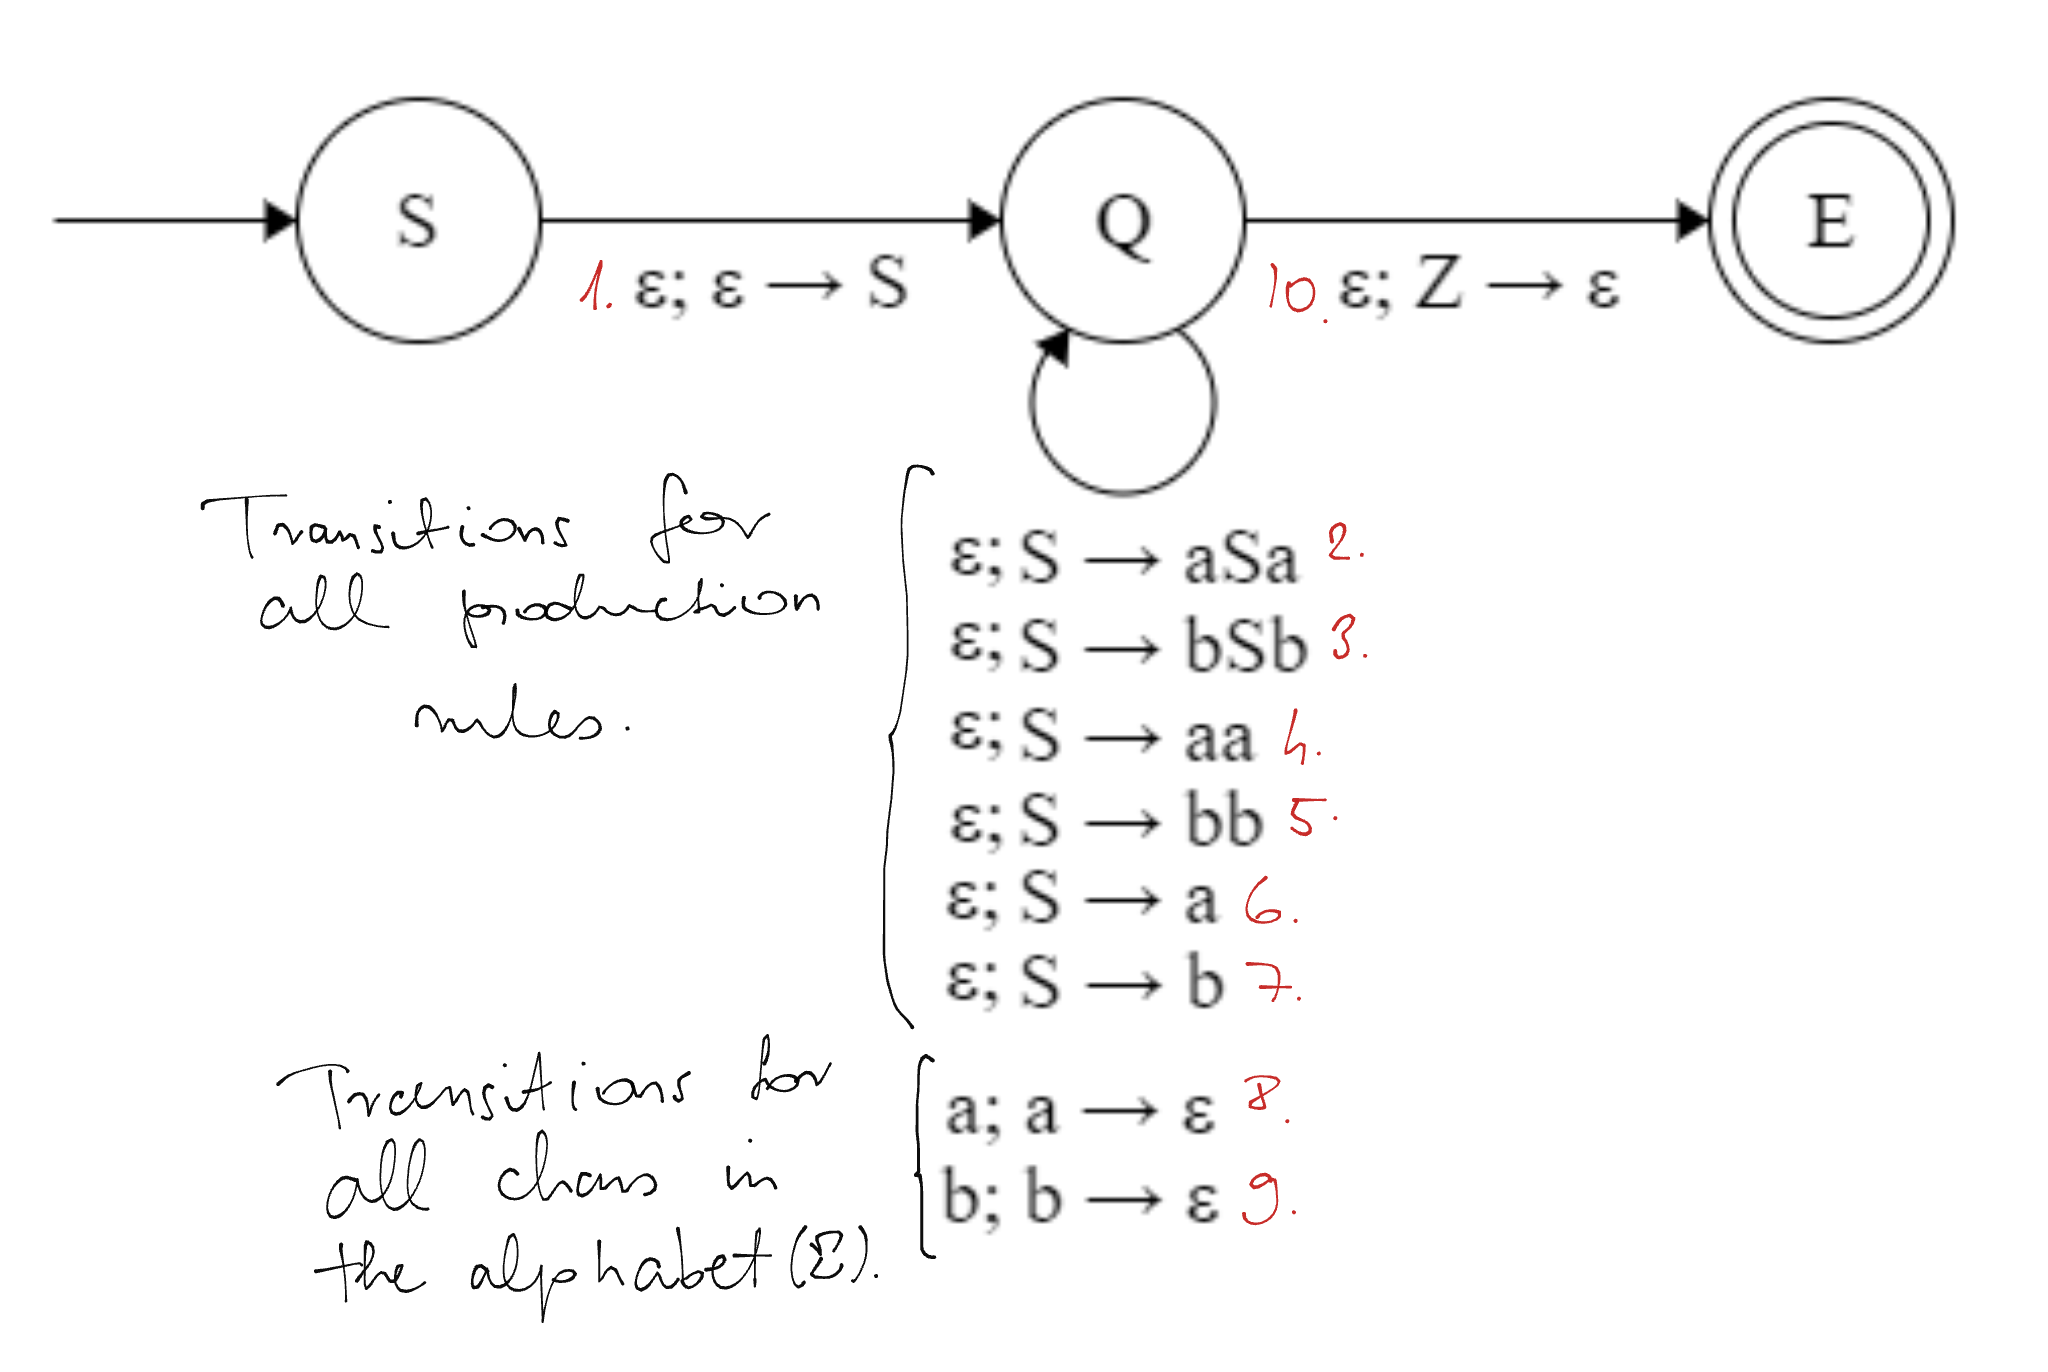
\includegraphics[width=\linewidth]{05/6_1.png}

\begin{itemize}
    \item Transition 1: First, we put the starting variable $S$ on top of the stack.
    \item Transitions 2-7: For all production rules in the grammar we add transitions, which will take care of doing the (leftmost) derivation inside the stack, while not reading from the input.
    \item Transitions 8-9: For all letters in the alphabet we add production rules, which will take care of comparing the input with the derived word in the stack.
    \item Transition 10: Finally we check if the stack is empty and only move to the accept state $E$ if it is.
\end{itemize}

b)

Accepting computation for $ababa$:

$(S, ababa, Z)
\xrightarrow{1.} (Q, ababa, SZ)
\xrightarrow{2.} (Q, ababa, aSaZ)
\xrightarrow{8.} (Q, baba, SaZ)
\xrightarrow{3.} (Q, baba, bSbaZ)
\xrightarrow{9.} (Q, aba, SbaZ)
\xrightarrow{6.} (Q, aba, abaZ)
\xrightarrow{8.} (Q, ba, baZ)
\xrightarrow{9.} (Q, a, aZ)
\xrightarrow{8.} (Q, \varepsilon, Z)
\xrightarrow{10.} (E, \varepsilon, \varepsilon)$
